\section{Tree Graph State}
\label{chap:tree_graph_state}
\thispagestyle{fancy}

The work by Y. Zhan \emph{et al.} \cite{tree_graph_state} highlighted the central challenge of reliably transmitting quantum signals through noisy and lossy channels.

While conventional quantum repeater proposals relied on heraled entanglement generation and two-way classical signaling, recent proposals have been made towards leveraging \emph{photonic graph states} to overcome these challenges.
These graph-state-based quantum repeaters \cite{One_way_quantum_repeaters} present a promising alternative by employing quantum encoding to address photon losses and operational errors, ultimately bypassing the necessity for extensive quantum memory coherence times.

However, generating such photonic graph states traditionally demands substantial resources and intricate methodologies involving linear optics and a considerable amounts of auxiliary qubits.
Despite this challenge, various schemes have been proposed for deterministic generation of these states, including \emph{tree graph} and \emph{repeater graph states}.

This section will look into how we can create these graph states using our device. 
In the previous sections, we have described the key steps to make specific types of graphs and entanglement bonds between the qubits in our device.
Now, we will explore how to use these tools to generate these graph states, with potential future applications in quantum networking.

\subsection{(2, 2) Tree Graph State}
\label{sec:2_2_tree}

\begin{figure}
    \centering
    

\tikzset{every picture/.style={line width=0.75pt}} %set default line width to 0.75pt        

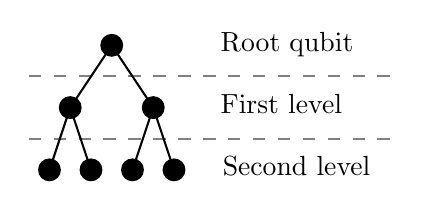
\begin{tikzpicture}[x=0.75pt,y=0.75pt,yscale=-1,xscale=1]
%uncomment if require: \path (0,300); %set diagram left start at 0, and has height of 300

%Straight Lines [id:da8426905590991587] 
\draw [color={rgb, 255:red, 128; green, 128; blue, 128 }  ,draw opacity=1 ] [dash pattern={on 4.5pt off 4.5pt}]  (60,85) -- (240,85) ;
%Straight Lines [id:da5406148798931413] 
\draw [color={rgb, 255:red, 128; green, 128; blue, 128 }  ,draw opacity=1 ] [dash pattern={on 4.5pt off 4.5pt}]  (60,55) -- (240,55) ;
%Straight Lines [id:da0310472865739988] 
\draw    (80,70) -- (90,100) ;
%Straight Lines [id:da44724908569705224] 
\draw    (80,70) -- (100,40) ;
%Shape: Circle [id:dp9646050192410193] 
\draw  [fill={rgb, 255:red, 0; green, 0; blue, 0 }  ,fill opacity=1 ] (95,40) .. controls (95,37.24) and (97.24,35) .. (100,35) .. controls (102.76,35) and (105,37.24) .. (105,40) .. controls (105,42.76) and (102.76,45) .. (100,45) .. controls (97.24,45) and (95,42.76) .. (95,40) -- cycle ;
%Shape: Circle [id:dp9987430184128605] 
\draw  [fill={rgb, 255:red, 0; green, 0; blue, 0 }  ,fill opacity=1 ] (105,100) .. controls (105,97.24) and (107.24,95) .. (110,95) .. controls (112.76,95) and (115,97.24) .. (115,100) .. controls (115,102.76) and (112.76,105) .. (110,105) .. controls (107.24,105) and (105,102.76) .. (105,100) -- cycle ;
%Shape: Circle [id:dp5327923177036115] 
\draw  [fill={rgb, 255:red, 0; green, 0; blue, 0 }  ,fill opacity=1 ] (125,100) .. controls (125,97.24) and (127.24,95) .. (130,95) .. controls (132.76,95) and (135,97.24) .. (135,100) .. controls (135,102.76) and (132.76,105) .. (130,105) .. controls (127.24,105) and (125,102.76) .. (125,100) -- cycle ;
%Shape: Circle [id:dp07874792740386194] 
\draw  [fill={rgb, 255:red, 0; green, 0; blue, 0 }  ,fill opacity=1 ] (115,70) .. controls (115,67.24) and (117.24,65) .. (120,65) .. controls (122.76,65) and (125,67.24) .. (125,70) .. controls (125,72.76) and (122.76,75) .. (120,75) .. controls (117.24,75) and (115,72.76) .. (115,70) -- cycle ;
%Shape: Circle [id:dp827553292195197] 
\draw  [fill={rgb, 255:red, 0; green, 0; blue, 0 }  ,fill opacity=1 ] (65,100) .. controls (65,97.24) and (67.24,95) .. (70,95) .. controls (72.76,95) and (75,97.24) .. (75,100) .. controls (75,102.76) and (72.76,105) .. (70,105) .. controls (67.24,105) and (65,102.76) .. (65,100) -- cycle ;
%Shape: Circle [id:dp9737971224660668] 
\draw  [fill={rgb, 255:red, 0; green, 0; blue, 0 }  ,fill opacity=1 ] (85,100) .. controls (85,97.24) and (87.24,95) .. (90,95) .. controls (92.76,95) and (95,97.24) .. (95,100) .. controls (95,102.76) and (92.76,105) .. (90,105) .. controls (87.24,105) and (85,102.76) .. (85,100) -- cycle ;
%Shape: Circle [id:dp3888180938045467] 
\draw  [fill={rgb, 255:red, 0; green, 0; blue, 0 }  ,fill opacity=1 ] (75,70) .. controls (75,67.24) and (77.24,65) .. (80,65) .. controls (82.76,65) and (85,67.24) .. (85,70) .. controls (85,72.76) and (82.76,75) .. (80,75) .. controls (77.24,75) and (75,72.76) .. (75,70) -- cycle ;
%Straight Lines [id:da09087177582110562] 
\draw    (80,70) -- (70,100) ;
%Straight Lines [id:da9701309593546271] 
\draw    (100,40) -- (120,70) ;
%Straight Lines [id:da7485547301936679] 
\draw    (110,100) -- (120,70) ;
%Straight Lines [id:da005037302745795835] 
\draw    (120,70) -- (130,100) ;

% Text Node
\draw (151,32) node [anchor=north west][inner sep=0.75pt]   [align=left] {Root qubit};
% Text Node
\draw (151,62) node [anchor=north west][inner sep=0.75pt]   [align=left] {First level};
% Text Node
\draw (152,92) node [anchor=north west][inner sep=0.75pt]   [align=left] {Second level};


\end{tikzpicture}
    \vspace{-1cm}
    \caption{Representation of $(2, 2)$ tree graph state}
    \label{fig:2_2_graph}
\end{figure}

The term \emph{$(n, m)$ tree graph state} refers to a tree structure where the initial qubit, known as the root qubit, links to $n$ other qubits, each of which is connected to $m$ additional qubits.
Specifically, we'll focus on examining a $(2, 2)$ tree graph state, visually represented in \cref{fig:2_2_graph}.

The tree graph state holds importance in one-way quantum repeater protocols as one can encode a logical state on the entire graph by running operations between a data qubit and the root node.
This resilience, requiring only a subset of essential photons for loss correction \cite{Why_tree_graph_state}, enables qubit transmission even if some photons are lost, ensuring reliable communication despite potential losses.
Hence, it is crucial to create the tree graph state while ensuring the root remains stored within one of our qubits, as it is necessary for Bell state measurements, enabling the encoding of the intended state for transmission.

We will begin by outlining the protocol employed to create the initial branch of the $(2, 2)$ tree graph state.
Initially, we generate the root qubit for the tree state using a straightforward $\pi/2$ $y$ rotation.
In the circuit diagram, the first quantum wire represents the root of the tree, stored within one of the physical qubits of our device.
The second quantum wire represents the second physical qubit, while the remaining wires symbolize flying photons.
\begin{equation}
\label{eq:1_branch_implementation}
    \begin{quantikz}
      \lstick{$\ket{0}_{S1}$} & \gate{Y_+}\slice[style=black]{\textbf{(a)}}  & \qw      & \qw  & \qw & \ctrl{1}  & \qw & \qw   & \qw      & \qw & \qw &  \qw & \qw & \qw \\
      \lstick{$\ket{0}_{S2}$} & \gate{Y_+} & \ctrl{1} & \gate{Y_-} \slice[style=black]{\textbf{(b)}} &  \qw   & \control{}  & \qw \slice[style=black]{\textbf{(c)}} & \qw   & \ctrl{2} & \gate{Y_+}\slice[style=black]{\textbf{(d)}} & \qw & \swap{3} & \qw \slice[style=black]{\textbf{(e)}} & \qw \\
      \lstick{$\ket{0}_{P1}$} & \qw                 & \targ{}      & \qw           & \qw       & \qw     & \qw   & \qw   & \qw  & \qw                 & \qw & \qw & \qw & \qw\\
      \lstick{$\ket{0}_{P2}$} & \qw                 & \qw          & \qw           & \qw       & \qw     & \qw   & \qw   & \targ{}      & \qw                 & \qw & \qw & \qw & \qw  \\
      \lstick{$\ket{0}_{P3}$} & \qw                 & \qw      & \qw          & \qw        & \qw      & \qw  & \qw   & \qw      & \qw                 & \qw & \targX{} & \qw & \qw
    \end{quantikz}
\end{equation}

\begin{figure}[b]
    \centering
    

\tikzset{every picture/.style={line width=0.75pt}} %set default line width to 0.75pt        

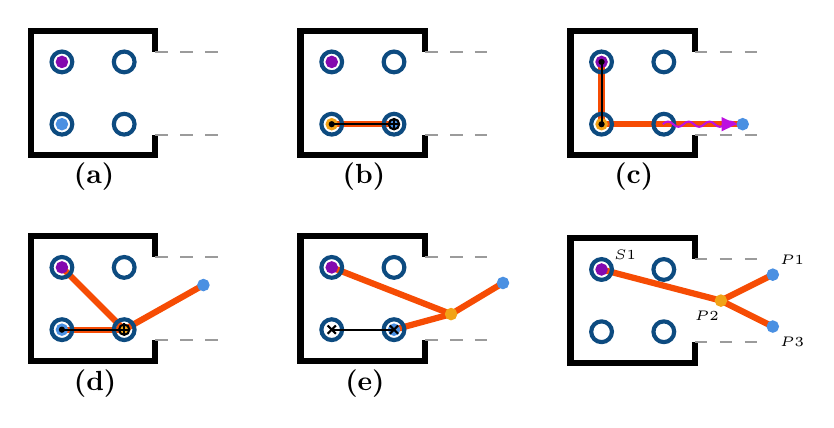
\begin{tikzpicture}[x=0.75pt,y=0.75pt,yscale=-1,xscale=1]
%uncomment if require: \path (0,223); %set diagram left start at 0, and has height of 223

%Shape: Square [id:dp8674749037525845] 
\draw  [line width=2.25]  (150,119) -- (210,119) -- (210,179) -- (150,179) -- cycle ;
%Straight Lines [id:da5545620865490668] 
\draw [color={rgb, 255:red, 255; green, 255; blue, 255 }  ,draw opacity=1 ][line width=3]    (210,129) -- (210,169) ;

%Shape: Circle [id:dp8634696649139634] 
\draw  [color={rgb, 255:red, 13; green, 75; blue, 128 }  ,draw opacity=1 ][line width=1.5]  (30,35) .. controls (30,32.24) and (32.24,30) .. (35,30) .. controls (37.76,30) and (40,32.24) .. (40,35) .. controls (40,37.76) and (37.76,40) .. (35,40) .. controls (32.24,40) and (30,37.76) .. (30,35) -- cycle ;
%Shape: Circle [id:dp3171229884283615] 
\draw  [color={rgb, 255:red, 13; green, 75; blue, 128 }  ,draw opacity=1 ][line width=1.5]  (30,65) .. controls (30,62.24) and (32.24,60) .. (35,60) .. controls (37.76,60) and (40,62.24) .. (40,65) .. controls (40,67.76) and (37.76,70) .. (35,70) .. controls (32.24,70) and (30,67.76) .. (30,65) -- cycle ;
%Shape: Circle [id:dp8674284799713297] 
\draw  [color={rgb, 255:red, 13; green, 75; blue, 128 }  ,draw opacity=1 ][line width=1.5]  (60,65) .. controls (60,62.24) and (62.24,60) .. (65,60) .. controls (67.76,60) and (70,62.24) .. (70,65) .. controls (70,67.76) and (67.76,70) .. (65,70) .. controls (62.24,70) and (60,67.76) .. (60,65) -- cycle ;
%Shape: Circle [id:dp13408530876145808] 
\draw  [color={rgb, 255:red, 13; green, 75; blue, 128 }  ,draw opacity=1 ][line width=1.5]  (60,35) .. controls (60,32.24) and (62.24,30) .. (65,30) .. controls (67.76,30) and (70,32.24) .. (70,35) .. controls (70,37.76) and (67.76,40) .. (65,40) .. controls (62.24,40) and (60,37.76) .. (60,35) -- cycle ;
%Shape: Square [id:dp47099491834906715] 
\draw  [line width=2.25]  (20,20) -- (80,20) -- (80,80) -- (20,80) -- cycle ;
%Straight Lines [id:da0834144987419978] 
\draw [color={rgb, 255:red, 255; green, 255; blue, 255 }  ,draw opacity=1 ][line width=3]    (80,30) -- (80,70) ;

%Shape: Circle [id:dp5113434790777113] 
\draw  [color={rgb, 255:red, 132; green, 9; blue, 175 }  ,draw opacity=1 ][fill={rgb, 255:red, 132; green, 9; blue, 175 }  ,fill opacity=1 ] (32.5,35) .. controls (32.5,33.62) and (33.62,32.5) .. (35,32.5) .. controls (36.38,32.5) and (37.5,33.62) .. (37.5,35) .. controls (37.5,36.38) and (36.38,37.5) .. (35,37.5) .. controls (33.62,37.5) and (32.5,36.38) .. (32.5,35) -- cycle ;
%Straight Lines [id:da46112915361915263] 
\draw [color={rgb, 255:red, 155; green, 155; blue, 155 }  ,draw opacity=1 ] [dash pattern={on 4.5pt off 4.5pt}]  (80,30) -- (110,30) ;
%Straight Lines [id:da9498457389457537] 
\draw [color={rgb, 255:red, 155; green, 155; blue, 155 }  ,draw opacity=1 ] [dash pattern={on 4.5pt off 4.5pt}]  (80,70) -- (110,70) ;
%Shape: Circle [id:dp9873280063938384] 
\draw  [color={rgb, 255:red, 74; green, 144; blue, 226 }  ,draw opacity=1 ][fill={rgb, 255:red, 74; green, 144; blue, 226 }  ,fill opacity=1 ] (32.5,65) .. controls (32.5,63.62) and (33.62,62.5) .. (35,62.5) .. controls (36.38,62.5) and (37.5,63.62) .. (37.5,65) .. controls (37.5,66.38) and (36.38,67.5) .. (35,67.5) .. controls (33.62,67.5) and (32.5,66.38) .. (32.5,65) -- cycle ;
%Shape: Circle [id:dp6431718269187471] 
\draw  [color={rgb, 255:red, 132; green, 9; blue, 175 }  ,draw opacity=1 ][fill={rgb, 255:red, 132; green, 9; blue, 175 }  ,fill opacity=1 ] (162.5,35) .. controls (162.5,33.62) and (163.62,32.5) .. (165,32.5) .. controls (166.38,32.5) and (167.5,33.62) .. (167.5,35) .. controls (167.5,36.38) and (166.38,37.5) .. (165,37.5) .. controls (163.62,37.5) and (162.5,36.38) .. (162.5,35) -- cycle ;
%Shape: Circle [id:dp21383549781911027] 
\draw  [color={rgb, 255:red, 13; green, 75; blue, 128 }  ,draw opacity=1 ][line width=1.5]  (160,35) .. controls (160,32.24) and (162.24,30) .. (165,30) .. controls (167.76,30) and (170,32.24) .. (170,35) .. controls (170,37.76) and (167.76,40) .. (165,40) .. controls (162.24,40) and (160,37.76) .. (160,35) -- cycle ;
%Shape: Circle [id:dp3789153251551227] 
\draw  [color={rgb, 255:red, 13; green, 75; blue, 128 }  ,draw opacity=1 ][line width=1.5]  (190,35) .. controls (190,32.24) and (192.24,30) .. (195,30) .. controls (197.76,30) and (200,32.24) .. (200,35) .. controls (200,37.76) and (197.76,40) .. (195,40) .. controls (192.24,40) and (190,37.76) .. (190,35) -- cycle ;
%Shape: Square [id:dp28884126483287875] 
\draw  [line width=2.25]  (150,20) -- (210,20) -- (210,80) -- (150,80) -- cycle ;
%Straight Lines [id:da7068966502224133] 
\draw [color={rgb, 255:red, 255; green, 255; blue, 255 }  ,draw opacity=1 ][line width=3]    (210,30) -- (210,70) ;

%Straight Lines [id:da5803960409811918] 
\draw [color={rgb, 255:red, 155; green, 155; blue, 155 }  ,draw opacity=1 ] [dash pattern={on 4.5pt off 4.5pt}]  (210,30) -- (240,30) ;
%Straight Lines [id:da7547530202356005] 
\draw [color={rgb, 255:red, 155; green, 155; blue, 155 }  ,draw opacity=1 ] [dash pattern={on 4.5pt off 4.5pt}]  (210,70) -- (240,70) ;
%Straight Lines [id:da6849475869613678] 
\draw [color={rgb, 255:red, 246; green, 76; blue, 4 }  ,draw opacity=1 ][line width=2.25]    (165,65) -- (195,65) ;
%Shape: Circle [id:dp7155137713689077] 
\draw  [color={rgb, 255:red, 241; green, 163; blue, 23 }  ,draw opacity=1 ][fill={rgb, 255:red, 241; green, 163; blue, 23 }  ,fill opacity=1 ] (162.5,65) .. controls (162.5,63.62) and (163.62,62.5) .. (165,62.5) .. controls (166.38,62.5) and (167.5,63.62) .. (167.5,65) .. controls (167.5,66.38) and (166.38,67.5) .. (165,67.5) .. controls (163.62,67.5) and (162.5,66.38) .. (162.5,65) -- cycle ;
%Shape: Circle [id:dp2190211775758546] 
\draw  [color={rgb, 255:red, 0; green, 0; blue, 0 }  ,draw opacity=1 ][fill={rgb, 255:red, 74; green, 144; blue, 226 }  ,fill opacity=1 ] (192.5,65) .. controls (192.5,63.62) and (193.62,62.5) .. (195,62.5) .. controls (196.38,62.5) and (197.5,63.62) .. (197.5,65) .. controls (197.5,66.38) and (196.38,67.5) .. (195,67.5) .. controls (193.62,67.5) and (192.5,66.38) .. (192.5,65) -- cycle ;
%Straight Lines [id:da5019530038163004] 
\draw    (195,62.5) -- (195,68) ;
%Straight Lines [id:da023533720970719596] 
\draw    (197.5,65) -- (192.5,65) ;
%Shape: Circle [id:dp463883226646705] 
\draw  [draw opacity=0][fill={rgb, 255:red, 0; green, 0; blue, 0 }  ,fill opacity=1 ] (163.5,65) .. controls (163.5,64.17) and (164.17,63.5) .. (165,63.5) .. controls (165.83,63.5) and (166.5,64.17) .. (166.5,65) .. controls (166.5,65.83) and (165.83,66.5) .. (165,66.5) .. controls (164.17,66.5) and (163.5,65.83) .. (163.5,65) -- cycle ;
%Shape: Circle [id:dp2941797335933385] 
\draw  [color={rgb, 255:red, 13; green, 75; blue, 128 }  ,draw opacity=1 ][line width=1.5]  (190,65) .. controls (190,62.24) and (192.24,60) .. (195,60) .. controls (197.76,60) and (200,62.24) .. (200,65) .. controls (200,67.76) and (197.76,70) .. (195,70) .. controls (192.24,70) and (190,67.76) .. (190,65) -- cycle ;
%Shape: Circle [id:dp19508965820109148] 
\draw  [color={rgb, 255:red, 13; green, 75; blue, 128 }  ,draw opacity=1 ][line width=1.5]  (160,65) .. controls (160,62.24) and (162.24,60) .. (165,60) .. controls (167.76,60) and (170,62.24) .. (170,65) .. controls (170,67.76) and (167.76,70) .. (165,70) .. controls (162.24,70) and (160,67.76) .. (160,65) -- cycle ;
%Straight Lines [id:da36230041238257815] 
\draw    (165,65) -- (195,65) ;
%Shape: Square [id:dp22566803032018268] 
\draw  [line width=2.25]  (280,20) -- (340,20) -- (340,80) -- (280,80) -- cycle ;
%Straight Lines [id:da8610306823319624] 
\draw [color={rgb, 255:red, 255; green, 255; blue, 255 }  ,draw opacity=1 ][line width=3]    (340,30) -- (340,70) ;

%Straight Lines [id:da9138577476417785] 
\draw [color={rgb, 255:red, 246; green, 76; blue, 4 }  ,draw opacity=1 ][line width=2.25]    (295,65) -- (363,65) ;
%Straight Lines [id:da9264747080487808] 
\draw [color={rgb, 255:red, 246; green, 76; blue, 4 }  ,draw opacity=1 ][line width=2.25]    (295,35) -- (295,65) ;
%Shape: Circle [id:dp826290588201388] 
\draw  [color={rgb, 255:red, 132; green, 9; blue, 175 }  ,draw opacity=1 ][fill={rgb, 255:red, 132; green, 9; blue, 175 }  ,fill opacity=1 ] (292.5,35) .. controls (292.5,33.62) and (293.62,32.5) .. (295,32.5) .. controls (296.38,32.5) and (297.5,33.62) .. (297.5,35) .. controls (297.5,36.38) and (296.38,37.5) .. (295,37.5) .. controls (293.62,37.5) and (292.5,36.38) .. (292.5,35) -- cycle ;
%Shape: Circle [id:dp9454665293887276] 
\draw  [color={rgb, 255:red, 13; green, 75; blue, 128 }  ,draw opacity=1 ][line width=1.5]  (290,35) .. controls (290,32.24) and (292.24,30) .. (295,30) .. controls (297.76,30) and (300,32.24) .. (300,35) .. controls (300,37.76) and (297.76,40) .. (295,40) .. controls (292.24,40) and (290,37.76) .. (290,35) -- cycle ;
%Shape: Circle [id:dp9678738407214998] 
\draw  [color={rgb, 255:red, 13; green, 75; blue, 128 }  ,draw opacity=1 ][line width=1.5]  (290,65) .. controls (290,62.24) and (292.24,60) .. (295,60) .. controls (297.76,60) and (300,62.24) .. (300,65) .. controls (300,67.76) and (297.76,70) .. (295,70) .. controls (292.24,70) and (290,67.76) .. (290,65) -- cycle ;
%Shape: Circle [id:dp11638652073637779] 
\draw  [color={rgb, 255:red, 13; green, 75; blue, 128 }  ,draw opacity=1 ][line width=1.5]  (320,65) .. controls (320,62.24) and (322.24,60) .. (325,60) .. controls (327.76,60) and (330,62.24) .. (330,65) .. controls (330,67.76) and (327.76,70) .. (325,70) .. controls (322.24,70) and (320,67.76) .. (320,65) -- cycle ;
%Shape: Circle [id:dp8846315373556948] 
\draw  [color={rgb, 255:red, 13; green, 75; blue, 128 }  ,draw opacity=1 ][line width=1.5]  (320,35) .. controls (320,32.24) and (322.24,30) .. (325,30) .. controls (327.76,30) and (330,32.24) .. (330,35) .. controls (330,37.76) and (327.76,40) .. (325,40) .. controls (322.24,40) and (320,37.76) .. (320,35) -- cycle ;
%Straight Lines [id:da15824455233757484] 
\draw [color={rgb, 255:red, 155; green, 155; blue, 155 }  ,draw opacity=1 ] [dash pattern={on 4.5pt off 4.5pt}]  (340,30) -- (370,30) ;
%Straight Lines [id:da08275578074384338] 
\draw [color={rgb, 255:red, 155; green, 155; blue, 155 }  ,draw opacity=1 ] [dash pattern={on 4.5pt off 4.5pt}]  (340,70) -- (370,70) ;
%Shape: Circle [id:dp4480793960053918] 
\draw  [color={rgb, 255:red, 241; green, 163; blue, 23 }  ,draw opacity=1 ][fill={rgb, 255:red, 241; green, 163; blue, 23 }  ,fill opacity=1 ] (292.5,65) .. controls (292.5,63.62) and (293.62,62.5) .. (295,62.5) .. controls (296.38,62.5) and (297.5,63.62) .. (297.5,65) .. controls (297.5,66.38) and (296.38,67.5) .. (295,67.5) .. controls (293.62,67.5) and (292.5,66.38) .. (292.5,65) -- cycle ;
%Shape: Circle [id:dp4701197125733043] 
\draw  [color={rgb, 255:red, 74; green, 144; blue, 226 }  ,draw opacity=1 ][fill={rgb, 255:red, 74; green, 144; blue, 226 }  ,fill opacity=1 ] (360.5,65) .. controls (360.5,63.62) and (361.62,62.5) .. (363,62.5) .. controls (364.38,62.5) and (365.5,63.62) .. (365.5,65) .. controls (365.5,66.38) and (364.38,67.5) .. (363,67.5) .. controls (361.62,67.5) and (360.5,66.38) .. (360.5,65) -- cycle ;
%Shape: Circle [id:dp36402367761201493] 
\draw  [draw opacity=0][fill={rgb, 255:red, 0; green, 0; blue, 0 }  ,fill opacity=1 ] (293.5,65) .. controls (293.5,64.17) and (294.17,63.5) .. (295,63.5) .. controls (295.83,63.5) and (296.5,64.17) .. (296.5,65) .. controls (296.5,65.83) and (295.83,66.5) .. (295,66.5) .. controls (294.17,66.5) and (293.5,65.83) .. (293.5,65) -- cycle ;
%Shape: Circle [id:dp7874046855771671] 
\draw  [draw opacity=0][fill={rgb, 255:red, 0; green, 0; blue, 0 }  ,fill opacity=1 ] (293.5,35) .. controls (293.5,34.17) and (294.17,33.5) .. (295,33.5) .. controls (295.83,33.5) and (296.5,34.17) .. (296.5,35) .. controls (296.5,35.83) and (295.83,36.5) .. (295,36.5) .. controls (294.17,36.5) and (293.5,35.83) .. (293.5,35) -- cycle ;
%Straight Lines [id:da2898778351352036] 
\draw    (295,35) -- (295,65) ;
%Straight Lines [id:da7752313531562761] 
\draw [color={rgb, 255:red, 189; green, 16; blue, 224 }  ,draw opacity=1 ]   (324.5,65) .. controls (326.17,63.33) and (327.83,63.33) .. (329.5,65) .. controls (331.17,66.67) and (332.83,66.67) .. (334.5,65) .. controls (336.17,63.33) and (337.83,63.33) .. (339.5,65) .. controls (341.17,66.67) and (342.83,66.67) .. (344.5,65) .. controls (346.17,63.33) and (347.83,63.33) .. (349.5,65) .. controls (351.17,66.67) and (352.83,66.67) .. (354.5,65) .. controls (356.17,63.33) and (357.83,63.33) .. (359.5,65) -- (360,65) -- (360,65) ;
%Straight Lines [id:da9446040288212432] 
\draw [color={rgb, 255:red, 189; green, 16; blue, 224 }  ,draw opacity=1 ]   (354.25,65) -- (357,65) ;
\draw [shift={(360,65)}, rotate = 180] [fill={rgb, 255:red, 189; green, 16; blue, 224 }  ,fill opacity=1 ][line width=0.08]  [draw opacity=0] (7.14,-3.43) -- (0,0) -- (7.14,3.43) -- cycle    ;
%Straight Lines [id:da4458315367718473] 
\draw [color={rgb, 255:red, 246; green, 76; blue, 4 }  ,draw opacity=1 ][line width=2.25]    (35,164) -- (65,164) ;
%Straight Lines [id:da6417507071495968] 
\draw [color={rgb, 255:red, 246; green, 76; blue, 4 }  ,draw opacity=1 ][line width=2.25]    (35,134) -- (65,164) ;
%Shape: Square [id:dp19892382898236483] 
\draw  [line width=2.25]  (20,119) -- (80,119) -- (80,179) -- (20,179) -- cycle ;
%Straight Lines [id:da8211154882339877] 
\draw [color={rgb, 255:red, 255; green, 255; blue, 255 }  ,draw opacity=1 ][line width=3]    (80,129) -- (80,169) ;

%Straight Lines [id:da1226594004392908] 
\draw [color={rgb, 255:red, 246; green, 76; blue, 4 }  ,draw opacity=1 ][line width=2.25]    (103.17,142.5) -- (65,164) ;
%Shape: Circle [id:dp25607475791662804] 
\draw  [color={rgb, 255:red, 132; green, 9; blue, 175 }  ,draw opacity=1 ][fill={rgb, 255:red, 132; green, 9; blue, 175 }  ,fill opacity=1 ] (32.5,134) .. controls (32.5,132.62) and (33.62,131.5) .. (35,131.5) .. controls (36.38,131.5) and (37.5,132.62) .. (37.5,134) .. controls (37.5,135.38) and (36.38,136.5) .. (35,136.5) .. controls (33.62,136.5) and (32.5,135.38) .. (32.5,134) -- cycle ;
%Shape: Circle [id:dp7472085667416201] 
\draw  [color={rgb, 255:red, 13; green, 75; blue, 128 }  ,draw opacity=1 ][line width=1.5]  (30,134) .. controls (30,131.24) and (32.24,129) .. (35,129) .. controls (37.76,129) and (40,131.24) .. (40,134) .. controls (40,136.76) and (37.76,139) .. (35,139) .. controls (32.24,139) and (30,136.76) .. (30,134) -- cycle ;
%Shape: Circle [id:dp6105247050154898] 
\draw  [color={rgb, 255:red, 13; green, 75; blue, 128 }  ,draw opacity=1 ][line width=1.5]  (30,164) .. controls (30,161.24) and (32.24,159) .. (35,159) .. controls (37.76,159) and (40,161.24) .. (40,164) .. controls (40,166.76) and (37.76,169) .. (35,169) .. controls (32.24,169) and (30,166.76) .. (30,164) -- cycle ;
%Shape: Circle [id:dp10304227171071978] 
\draw  [color={rgb, 255:red, 13; green, 75; blue, 128 }  ,draw opacity=1 ][line width=1.5]  (60,164) .. controls (60,161.24) and (62.24,159) .. (65,159) .. controls (67.76,159) and (70,161.24) .. (70,164) .. controls (70,166.76) and (67.76,169) .. (65,169) .. controls (62.24,169) and (60,166.76) .. (60,164) -- cycle ;
%Shape: Circle [id:dp4134298947687973] 
\draw  [color={rgb, 255:red, 13; green, 75; blue, 128 }  ,draw opacity=1 ][line width=1.5]  (60,134) .. controls (60,131.24) and (62.24,129) .. (65,129) .. controls (67.76,129) and (70,131.24) .. (70,134) .. controls (70,136.76) and (67.76,139) .. (65,139) .. controls (62.24,139) and (60,136.76) .. (60,134) -- cycle ;
%Straight Lines [id:da05857273260240248] 
\draw [color={rgb, 255:red, 155; green, 155; blue, 155 }  ,draw opacity=1 ] [dash pattern={on 4.5pt off 4.5pt}]  (80,129) -- (110,129) ;
%Straight Lines [id:da8515467099208363] 
\draw [color={rgb, 255:red, 155; green, 155; blue, 155 }  ,draw opacity=1 ] [dash pattern={on 4.5pt off 4.5pt}]  (80,169) -- (110,169) ;
%Shape: Circle [id:dp3385953242829104] 
\draw  [color={rgb, 255:red, 74; green, 144; blue, 226 }  ,draw opacity=1 ][fill={rgb, 255:red, 74; green, 144; blue, 226 }  ,fill opacity=1 ] (32.5,164) .. controls (32.5,162.62) and (33.62,161.5) .. (35,161.5) .. controls (36.38,161.5) and (37.5,162.62) .. (37.5,164) .. controls (37.5,165.38) and (36.38,166.5) .. (35,166.5) .. controls (33.62,166.5) and (32.5,165.38) .. (32.5,164) -- cycle ;
%Shape: Circle [id:dp6520838784850642] 
\draw  [color={rgb, 255:red, 0; green, 0; blue, 0 }  ,draw opacity=1 ][fill={rgb, 255:red, 241; green, 163; blue, 23 }  ,fill opacity=1 ] (62.5,164) .. controls (62.5,162.62) and (63.62,161.5) .. (65,161.5) .. controls (66.38,161.5) and (67.5,162.62) .. (67.5,164) .. controls (67.5,165.38) and (66.38,166.5) .. (65,166.5) .. controls (63.62,166.5) and (62.5,165.38) .. (62.5,164) -- cycle ;
%Straight Lines [id:da9256744917784654] 
\draw    (65,161) -- (65,166.5) ;
%Straight Lines [id:da28871784610038775] 
\draw    (35,164) -- (65,164) ;
%Straight Lines [id:da9178977220598342] 
\draw    (67.5,164) -- (62.5,164) ;
%Shape: Circle [id:dp7957363186924172] 
\draw  [draw opacity=0][fill={rgb, 255:red, 0; green, 0; blue, 0 }  ,fill opacity=1 ] (33.5,164) .. controls (33.5,163.17) and (34.17,162.5) .. (35,162.5) .. controls (35.83,162.5) and (36.5,163.17) .. (36.5,164) .. controls (36.5,164.83) and (35.83,165.5) .. (35,165.5) .. controls (34.17,165.5) and (33.5,164.83) .. (33.5,164) -- cycle ;
%Shape: Circle [id:dp6977350768470425] 
\draw  [color={rgb, 255:red, 74; green, 144; blue, 226 }  ,draw opacity=1 ][fill={rgb, 255:red, 74; green, 144; blue, 226 }  ,fill opacity=1 ] (100.67,142.5) .. controls (100.67,141.12) and (101.79,140) .. (103.17,140) .. controls (104.55,140) and (105.67,141.12) .. (105.67,142.5) .. controls (105.67,143.88) and (104.55,145) .. (103.17,145) .. controls (101.79,145) and (100.67,143.88) .. (100.67,142.5) -- cycle ;
%Straight Lines [id:da36281393869691037] 
\draw [color={rgb, 255:red, 246; green, 76; blue, 4 }  ,draw opacity=1 ][line width=2.25]    (195,164) -- (222.5,156.5) ;
%Straight Lines [id:da7527509800509908] 
\draw [color={rgb, 255:red, 246; green, 76; blue, 4 }  ,draw opacity=1 ][line width=2.25]    (165,134) -- (222.5,156.5) ;
%Straight Lines [id:da7082074246436685] 
\draw [color={rgb, 255:red, 246; green, 76; blue, 4 }  ,draw opacity=1 ][line width=2.25]    (247.5,141.5) -- (222.5,156.5) ;
%Shape: Circle [id:dp07974527817408228] 
\draw  [color={rgb, 255:red, 132; green, 9; blue, 175 }  ,draw opacity=1 ][fill={rgb, 255:red, 132; green, 9; blue, 175 }  ,fill opacity=1 ] (162.5,134) .. controls (162.5,132.62) and (163.62,131.5) .. (165,131.5) .. controls (166.38,131.5) and (167.5,132.62) .. (167.5,134) .. controls (167.5,135.38) and (166.38,136.5) .. (165,136.5) .. controls (163.62,136.5) and (162.5,135.38) .. (162.5,134) -- cycle ;
%Shape: Circle [id:dp775415723535786] 
\draw  [color={rgb, 255:red, 13; green, 75; blue, 128 }  ,draw opacity=1 ][line width=1.5]  (160,134) .. controls (160,131.24) and (162.24,129) .. (165,129) .. controls (167.76,129) and (170,131.24) .. (170,134) .. controls (170,136.76) and (167.76,139) .. (165,139) .. controls (162.24,139) and (160,136.76) .. (160,134) -- cycle ;
%Shape: Circle [id:dp7762958624527873] 
\draw  [color={rgb, 255:red, 13; green, 75; blue, 128 }  ,draw opacity=1 ][line width=1.5]  (160,164) .. controls (160,161.24) and (162.24,159) .. (165,159) .. controls (167.76,159) and (170,161.24) .. (170,164) .. controls (170,166.76) and (167.76,169) .. (165,169) .. controls (162.24,169) and (160,166.76) .. (160,164) -- cycle ;
%Shape: Circle [id:dp3388097761852541] 
\draw  [color={rgb, 255:red, 13; green, 75; blue, 128 }  ,draw opacity=1 ][line width=1.5]  (190,164) .. controls (190,161.24) and (192.24,159) .. (195,159) .. controls (197.76,159) and (200,161.24) .. (200,164) .. controls (200,166.76) and (197.76,169) .. (195,169) .. controls (192.24,169) and (190,166.76) .. (190,164) -- cycle ;
%Shape: Circle [id:dp12179684438001948] 
\draw  [color={rgb, 255:red, 13; green, 75; blue, 128 }  ,draw opacity=1 ][line width=1.5]  (190,134) .. controls (190,131.24) and (192.24,129) .. (195,129) .. controls (197.76,129) and (200,131.24) .. (200,134) .. controls (200,136.76) and (197.76,139) .. (195,139) .. controls (192.24,139) and (190,136.76) .. (190,134) -- cycle ;
%Straight Lines [id:da621649400731312] 
\draw [color={rgb, 255:red, 155; green, 155; blue, 155 }  ,draw opacity=1 ] [dash pattern={on 4.5pt off 4.5pt}]  (210,129) -- (240,129) ;
%Straight Lines [id:da5146835836320703] 
\draw [color={rgb, 255:red, 155; green, 155; blue, 155 }  ,draw opacity=1 ] [dash pattern={on 4.5pt off 4.5pt}]  (210,169) -- (240,169) ;
%Shape: Circle [id:dp3915773980253143] 
\draw  [color={rgb, 255:red, 74; green, 144; blue, 226 }  ,draw opacity=1 ][fill={rgb, 255:red, 74; green, 144; blue, 226 }  ,fill opacity=1 ] (192.5,164) .. controls (192.5,162.62) and (193.62,161.5) .. (195,161.5) .. controls (196.38,161.5) and (197.5,162.62) .. (197.5,164) .. controls (197.5,165.38) and (196.38,166.5) .. (195,166.5) .. controls (193.62,166.5) and (192.5,165.38) .. (192.5,164) -- cycle ;
%Shape: Circle [id:dp683326593934911] 
\draw  [color={rgb, 255:red, 241; green, 163; blue, 23 }  ,draw opacity=1 ][fill={rgb, 255:red, 241; green, 163; blue, 23 }  ,fill opacity=1 ] (220,156.5) .. controls (220,155.12) and (221.12,154) .. (222.5,154) .. controls (223.88,154) and (225,155.12) .. (225,156.5) .. controls (225,157.88) and (223.88,159) .. (222.5,159) .. controls (221.12,159) and (220,157.88) .. (220,156.5) -- cycle ;
%Shape: Circle [id:dp1476686818284596] 
\draw  [color={rgb, 255:red, 74; green, 144; blue, 226 }  ,draw opacity=1 ][fill={rgb, 255:red, 74; green, 144; blue, 226 }  ,fill opacity=1 ] (245,141.5) .. controls (245,140.12) and (246.12,139) .. (247.5,139) .. controls (248.88,139) and (250,140.12) .. (250,141.5) .. controls (250,142.88) and (248.88,144) .. (247.5,144) .. controls (246.12,144) and (245,142.88) .. (245,141.5) -- cycle ;
%Straight Lines [id:da6806064341044397] 
\draw    (193,162) -- (197,166) ;
%Straight Lines [id:da28321943830045837] 
\draw    (197,162) -- (193,166) ;
%Straight Lines [id:da6882302053042542] 
\draw    (167,162) -- (163,166) ;
%Straight Lines [id:da040927876955351716] 
\draw    (163,162) -- (167,166) ;
%Straight Lines [id:da40880985508449363] 
\draw    (165,164) -- (195,164) ;
%Shape: Square [id:dp35339551764788013] 
\draw  [line width=2.25]  (280,120) -- (340,120) -- (340,180) -- (280,180) -- cycle ;
%Straight Lines [id:da6922995078099995] 
\draw [color={rgb, 255:red, 255; green, 255; blue, 255 }  ,draw opacity=1 ][line width=3]    (340,130) -- (340,170) ;

%Straight Lines [id:da9038263726774028] 
\draw [color={rgb, 255:red, 246; green, 76; blue, 4 }  ,draw opacity=1 ][line width=2.25]    (377.5,162.5) -- (352.5,150) ;
%Straight Lines [id:da8979943609034058] 
\draw [color={rgb, 255:red, 246; green, 76; blue, 4 }  ,draw opacity=1 ][line width=2.25]    (295,135) -- (352.5,150) ;
%Straight Lines [id:da6305591498834828] 
\draw [color={rgb, 255:red, 246; green, 76; blue, 4 }  ,draw opacity=1 ][line width=2.25]    (377.5,137.5) -- (352.5,150) ;
%Shape: Circle [id:dp8884018399903687] 
\draw  [color={rgb, 255:red, 132; green, 9; blue, 175 }  ,draw opacity=1 ][fill={rgb, 255:red, 132; green, 9; blue, 175 }  ,fill opacity=1 ] (292.5,135) .. controls (292.5,133.62) and (293.62,132.5) .. (295,132.5) .. controls (296.38,132.5) and (297.5,133.62) .. (297.5,135) .. controls (297.5,136.38) and (296.38,137.5) .. (295,137.5) .. controls (293.62,137.5) and (292.5,136.38) .. (292.5,135) -- cycle ;
%Shape: Circle [id:dp7875286506272443] 
\draw  [color={rgb, 255:red, 13; green, 75; blue, 128 }  ,draw opacity=1 ][line width=1.5]  (290,135) .. controls (290,132.24) and (292.24,130) .. (295,130) .. controls (297.76,130) and (300,132.24) .. (300,135) .. controls (300,137.76) and (297.76,140) .. (295,140) .. controls (292.24,140) and (290,137.76) .. (290,135) -- cycle ;
%Shape: Circle [id:dp12145260393054702] 
\draw  [color={rgb, 255:red, 13; green, 75; blue, 128 }  ,draw opacity=1 ][line width=1.5]  (290,165) .. controls (290,162.24) and (292.24,160) .. (295,160) .. controls (297.76,160) and (300,162.24) .. (300,165) .. controls (300,167.76) and (297.76,170) .. (295,170) .. controls (292.24,170) and (290,167.76) .. (290,165) -- cycle ;
%Shape: Circle [id:dp2261942451396799] 
\draw  [color={rgb, 255:red, 13; green, 75; blue, 128 }  ,draw opacity=1 ][line width=1.5]  (320,165) .. controls (320,162.24) and (322.24,160) .. (325,160) .. controls (327.76,160) and (330,162.24) .. (330,165) .. controls (330,167.76) and (327.76,170) .. (325,170) .. controls (322.24,170) and (320,167.76) .. (320,165) -- cycle ;
%Shape: Circle [id:dp9337691364868046] 
\draw  [color={rgb, 255:red, 13; green, 75; blue, 128 }  ,draw opacity=1 ][line width=1.5]  (320,135) .. controls (320,132.24) and (322.24,130) .. (325,130) .. controls (327.76,130) and (330,132.24) .. (330,135) .. controls (330,137.76) and (327.76,140) .. (325,140) .. controls (322.24,140) and (320,137.76) .. (320,135) -- cycle ;
%Straight Lines [id:da8123399178176031] 
\draw [color={rgb, 255:red, 155; green, 155; blue, 155 }  ,draw opacity=1 ] [dash pattern={on 4.5pt off 4.5pt}]  (340,130) -- (370,130) ;
%Straight Lines [id:da6206241139577952] 
\draw [color={rgb, 255:red, 155; green, 155; blue, 155 }  ,draw opacity=1 ] [dash pattern={on 4.5pt off 4.5pt}]  (340,170) -- (370,170) ;
%Shape: Circle [id:dp8328823250944828] 
\draw  [color={rgb, 255:red, 74; green, 144; blue, 226 }  ,draw opacity=1 ][fill={rgb, 255:red, 74; green, 144; blue, 226 }  ,fill opacity=1 ] (375,162.5) .. controls (375,161.12) and (376.12,160) .. (377.5,160) .. controls (378.88,160) and (380,161.12) .. (380,162.5) .. controls (380,163.88) and (378.88,165) .. (377.5,165) .. controls (376.12,165) and (375,163.88) .. (375,162.5) -- cycle ;
%Shape: Circle [id:dp5040180519242364] 
\draw  [color={rgb, 255:red, 241; green, 163; blue, 23 }  ,draw opacity=1 ][fill={rgb, 255:red, 241; green, 163; blue, 23 }  ,fill opacity=1 ] (350,150) .. controls (350,148.62) and (351.12,147.5) .. (352.5,147.5) .. controls (353.88,147.5) and (355,148.62) .. (355,150) .. controls (355,151.38) and (353.88,152.5) .. (352.5,152.5) .. controls (351.12,152.5) and (350,151.38) .. (350,150) -- cycle ;
%Shape: Circle [id:dp840403992255841] 
\draw  [color={rgb, 255:red, 74; green, 144; blue, 226 }  ,draw opacity=1 ][fill={rgb, 255:red, 74; green, 144; blue, 226 }  ,fill opacity=1 ] (375,137.5) .. controls (375,136.12) and (376.12,135) .. (377.5,135) .. controls (378.88,135) and (380,136.12) .. (380,137.5) .. controls (380,138.88) and (378.88,140) .. (377.5,140) .. controls (376.12,140) and (375,138.88) .. (375,137.5) -- cycle ;

% Text Node
\draw (50.5,82) node [anchor=north] [inner sep=0.75pt]   [align=left] {\textbf{(a)}};
% Text Node
\draw (180.5,82) node [anchor=north] [inner sep=0.75pt]   [align=left] {\textbf{(b)}};
% Text Node
\draw (310.5,82) node [anchor=north] [inner sep=0.75pt]   [align=left] {\textbf{(c)}};
% Text Node
\draw (51,182) node [anchor=north] [inner sep=0.75pt]   [align=left] {\textbf{(d)}};
% Text Node
\draw (181,182) node [anchor=north] [inner sep=0.75pt]   [align=left] {\textbf{(e)}};
% Text Node
\draw (299.5,131.6) node [anchor=south west] [inner sep=0.75pt]  [font=\tiny]  {$S1$};
% Text Node
\draw (379.5,134.1) node [anchor=south west] [inner sep=0.75pt]  [font=\tiny]  {$P1$};
% Text Node
\draw (353,153.4) node [anchor=north east] [inner sep=0.75pt]  [font=\tiny]  {$P2$};
% Text Node
\draw (379.5,165.9) node [anchor=north west][inner sep=0.75pt]  [font=\tiny]  {$P3$};


\end{tikzpicture}
    \vspace{-1cm}
    \caption{Visual implementation of first branch of the $(2, 2)$ tree graph state}
    \label{fig:1_branch_tree}
\end{figure}

Fig.~\ref{fig:1_branch_tree} illustrates the visual progression occurring within the device.

Should we emit all nodes except for the root, we can replicate the process to generate the second and final branch of the intended quantum state.
The circuit illustrating the entire implementation of the tree graph state is presented below. 
Notably, the initial two quantum wires maintain their role as the first and second storage qubits.
Meanwhile, the remaining six wires signify the six additional vertices in the state, functioning as flying qubits in our configuration.
\begin{equation}
\label{eq:tree_implementation}
    \begin{quantikz}[column sep=0.4cm]
      \lstick{$\ket{0}_{S1}$} & \gate{Y_+} & \qw & \qw & \ctrl{1} & \qw & \qw & \qw & \qw & \qw & \qw & \ctrl{1} & \qw & \qw & \qw & \qw \\
      \lstick{$\ket{0}_{S2}$} & \gate{Y_+} & \ctrl{1} & \gate{Y_-} & \control{} & \ctrl{2} & \gate{Y_+} & \swap{3} & \gate{Y_+} & \ctrl{4} & \gate{Y_-} & \control{} & \ctrl{5} & \gate{Y_+} & \swap{6} & \qw \\
      \lstick{$\ket{0}_{P1}$} & \qw & \targ{} & \qw & \qw & \qw & \qw & \qw & \qw & \qw & \qw & \qw & \qw & \qw & \qw & \qw \\
      \lstick{$\ket{0}_{P2}$} & \qw & \qw & \qw & \qw & \targ{} & \qw & \qw & \qw & \qw & \qw & \qw & \qw & \qw & \qw & \qw \\
      \lstick{$\ket{0}_{P3}$} & \qw & \qw & \qw & \qw & \qw & \qw & \targX{} & \qw & \qw & \qw & \qw & \qw & \qw & \qw & \qw \\
      \lstick{$\ket{0}_{P4}$} & \qw & \qw & \qw & \qw & \qw & \qw & \qw & \qw & \targ{} & \qw & \qw & \qw & \qw & \qw & \qw \\
      \lstick{$\ket{0}_{P5}$} & \qw & \qw & \qw & \qw & \qw & \qw & \qw & \qw & \qw & \qw & \qw & \targ{} & \qw & \qw & \qw \\
      \lstick{$\ket{0}_{P6}$} & \qw & \qw & \qw & \qw & \qw & \qw & \qw & \qw & \qw & \qw & \qw & \qw & \qw & \targX{} & \qw
    \end{quantikz}
\end{equation}

The state generated with the previous circuit is equivalent to the following graph state.

\begin{equation}
\label{eq:tree_graph_state}
    \begin{quantikz}
        \lstick{$\ket{0}_{S1}$} & \gate{H}  & \ctrl{2}  & \qw  & \qw  & \ctrl{5}  & \qw  & \qw  & \qw \\
        \lstick{$\ket{0}_{P1}$} & \gate{H}  & \qw  & \qw  & \ctrl{1}  & \qw  & \qw  & \qw  & \qw \\
        \lstick{$\ket{0}_{P2}$} & \gate{H}  & \control{}  & \ctrl{1}  & \control{}  & \qw  & \qw  & \qw  & \qw \\
        \lstick{$\ket{0}_{P3}$} & \gate{H}  & \qw  & \control{}  & \qw  & \qw  & \qw  & \qw  & \qw \\
        \lstick{$\ket{0}_{P4}$} & \gate{H}  & \qw  & \qw  & \qw  & \qw  & \qw  & \ctrl{1}  & \qw \\
        \lstick{$\ket{0}_{P5}$} & \gate{H}  & \qw  & \qw  & \qw  & \control{}  & \ctrl{1}  & \control{}  & \qw \\
        \lstick{$\ket{0}_{P6}$} & \gate{H}  & \qw  & \qw  & \qw  & \qw  & \control{}  & \qw  & \qw
    \end{quantikz}
\end{equation}

Fig.~\ref{fig:final_tree_implementation} shows the final state we would get if we were to implement \cref{eq:tree_implementation} on our device, labelling the vertices according to the numbering in the equation.

% \begin{figure}
%     \centering
%     

\tikzset{every picture/.style={line width=0.75pt}} %set default line width to 0.75pt        

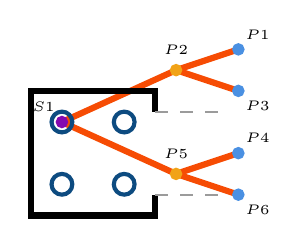
\begin{tikzpicture}[x=0.75pt,y=0.75pt,yscale=-1,xscale=1]
%uncomment if require: \path (0,182); %set diagram left start at 0, and has height of 182

%Straight Lines [id:da47465656152714486] 
\draw [color={rgb, 255:red, 246; green, 76; blue, 4 }  ,draw opacity=1 ][line width=2.25]    (315,75) -- (370,50) ;
%Shape: Square [id:dp7338884259497895] 
\draw  [line width=2.25]  (300,60) -- (360,60) -- (360,120) -- (300,120) -- cycle ;
%Straight Lines [id:da6927342142359094] 
\draw [color={rgb, 255:red, 255; green, 255; blue, 255 }  ,draw opacity=1 ][line width=3]    (360,70) -- (360,110) ;

%Straight Lines [id:da6098087629891208] 
\draw [color={rgb, 255:red, 246; green, 76; blue, 4 }  ,draw opacity=1 ][line width=2.25]    (370,50) -- (400,60) ;
%Straight Lines [id:da9586171017662504] 
\draw [color={rgb, 255:red, 246; green, 76; blue, 4 }  ,draw opacity=1 ][line width=2.25]    (400,40) -- (370,50) ;
%Straight Lines [id:da9166685119570428] 
\draw [color={rgb, 255:red, 246; green, 76; blue, 4 }  ,draw opacity=1 ][line width=2.25]    (370,100) -- (400,110) ;
%Straight Lines [id:da12081008351293132] 
\draw [color={rgb, 255:red, 246; green, 76; blue, 4 }  ,draw opacity=1 ][line width=2.25]    (315,75) -- (370,100) ;
%Straight Lines [id:da43191174777453967] 
\draw [color={rgb, 255:red, 246; green, 76; blue, 4 }  ,draw opacity=1 ][line width=2.25]    (400,90) -- (370,100) ;
%Shape: Circle [id:dp41145059566786146] 
\draw  [color={rgb, 255:red, 132; green, 9; blue, 175 }  ,draw opacity=1 ][fill={rgb, 255:red, 132; green, 9; blue, 175 }  ,fill opacity=1 ] (312.5,75) .. controls (312.5,73.62) and (313.62,72.5) .. (315,72.5) .. controls (316.38,72.5) and (317.5,73.62) .. (317.5,75) .. controls (317.5,76.38) and (316.38,77.5) .. (315,77.5) .. controls (313.62,77.5) and (312.5,76.38) .. (312.5,75) -- cycle ;
%Shape: Circle [id:dp5320458710332802] 
\draw  [color={rgb, 255:red, 13; green, 75; blue, 128 }  ,draw opacity=1 ][line width=1.5]  (310,75) .. controls (310,72.24) and (312.24,70) .. (315,70) .. controls (317.76,70) and (320,72.24) .. (320,75) .. controls (320,77.76) and (317.76,80) .. (315,80) .. controls (312.24,80) and (310,77.76) .. (310,75) -- cycle ;
%Shape: Circle [id:dp3617334287188755] 
\draw  [color={rgb, 255:red, 13; green, 75; blue, 128 }  ,draw opacity=1 ][line width=1.5]  (310,105) .. controls (310,102.24) and (312.24,100) .. (315,100) .. controls (317.76,100) and (320,102.24) .. (320,105) .. controls (320,107.76) and (317.76,110) .. (315,110) .. controls (312.24,110) and (310,107.76) .. (310,105) -- cycle ;
%Shape: Circle [id:dp07731016955749404] 
\draw  [color={rgb, 255:red, 13; green, 75; blue, 128 }  ,draw opacity=1 ][line width=1.5]  (340,105) .. controls (340,102.24) and (342.24,100) .. (345,100) .. controls (347.76,100) and (350,102.24) .. (350,105) .. controls (350,107.76) and (347.76,110) .. (345,110) .. controls (342.24,110) and (340,107.76) .. (340,105) -- cycle ;
%Shape: Circle [id:dp16339127645713447] 
\draw  [color={rgb, 255:red, 13; green, 75; blue, 128 }  ,draw opacity=1 ][line width=1.5]  (340,75) .. controls (340,72.24) and (342.24,70) .. (345,70) .. controls (347.76,70) and (350,72.24) .. (350,75) .. controls (350,77.76) and (347.76,80) .. (345,80) .. controls (342.24,80) and (340,77.76) .. (340,75) -- cycle ;
%Straight Lines [id:da6337075775283348] 
\draw [color={rgb, 255:red, 155; green, 155; blue, 155 }  ,draw opacity=1 ] [dash pattern={on 4.5pt off 4.5pt}]  (360,70) -- (390,70) ;
%Straight Lines [id:da4062260044648891] 
\draw [color={rgb, 255:red, 155; green, 155; blue, 155 }  ,draw opacity=1 ] [dash pattern={on 4.5pt off 4.5pt}]  (360,110) -- (390,110) ;
%Shape: Circle [id:dp34879830519151855] 
\draw  [color={rgb, 255:red, 74; green, 144; blue, 226 }  ,draw opacity=1 ][fill={rgb, 255:red, 74; green, 144; blue, 226 }  ,fill opacity=1 ] (397.5,110) .. controls (397.5,108.62) and (398.62,107.5) .. (400,107.5) .. controls (401.38,107.5) and (402.5,108.62) .. (402.5,110) .. controls (402.5,111.38) and (401.38,112.5) .. (400,112.5) .. controls (398.62,112.5) and (397.5,111.38) .. (397.5,110) -- cycle ;
%Shape: Circle [id:dp05200913272998542] 
\draw  [color={rgb, 255:red, 241; green, 163; blue, 23 }  ,draw opacity=1 ][fill={rgb, 255:red, 241; green, 163; blue, 23 }  ,fill opacity=1 ] (367.5,100) .. controls (367.5,98.62) and (368.62,97.5) .. (370,97.5) .. controls (371.38,97.5) and (372.5,98.62) .. (372.5,100) .. controls (372.5,101.38) and (371.38,102.5) .. (370,102.5) .. controls (368.62,102.5) and (367.5,101.38) .. (367.5,100) -- cycle ;
%Shape: Circle [id:dp43357034961897] 
\draw  [color={rgb, 255:red, 74; green, 144; blue, 226 }  ,draw opacity=1 ][fill={rgb, 255:red, 74; green, 144; blue, 226 }  ,fill opacity=1 ] (397.5,40) .. controls (397.5,38.62) and (398.62,37.5) .. (400,37.5) .. controls (401.38,37.5) and (402.5,38.62) .. (402.5,40) .. controls (402.5,41.38) and (401.38,42.5) .. (400,42.5) .. controls (398.62,42.5) and (397.5,41.38) .. (397.5,40) -- cycle ;
%Shape: Circle [id:dp7842924247669173] 
\draw  [color={rgb, 255:red, 241; green, 163; blue, 23 }  ,draw opacity=1 ][fill={rgb, 255:red, 241; green, 163; blue, 23 }  ,fill opacity=1 ] (367.5,50) .. controls (367.5,48.62) and (368.62,47.5) .. (370,47.5) .. controls (371.38,47.5) and (372.5,48.62) .. (372.5,50) .. controls (372.5,51.38) and (371.38,52.5) .. (370,52.5) .. controls (368.62,52.5) and (367.5,51.38) .. (367.5,50) -- cycle ;
%Shape: Circle [id:dp5315495156196338] 
\draw  [color={rgb, 255:red, 74; green, 144; blue, 226 }  ,draw opacity=1 ][fill={rgb, 255:red, 74; green, 144; blue, 226 }  ,fill opacity=1 ] (397.5,60) .. controls (397.5,58.62) and (398.62,57.5) .. (400,57.5) .. controls (401.38,57.5) and (402.5,58.62) .. (402.5,60) .. controls (402.5,61.38) and (401.38,62.5) .. (400,62.5) .. controls (398.62,62.5) and (397.5,61.38) .. (397.5,60) -- cycle ;
%Shape: Circle [id:dp9788740260400791] 
\draw  [color={rgb, 255:red, 74; green, 144; blue, 226 }  ,draw opacity=1 ][fill={rgb, 255:red, 74; green, 144; blue, 226 }  ,fill opacity=1 ] (397.5,90) .. controls (397.5,88.62) and (398.62,87.5) .. (400,87.5) .. controls (401.38,87.5) and (402.5,88.62) .. (402.5,90) .. controls (402.5,91.38) and (401.38,92.5) .. (400,92.5) .. controls (398.62,92.5) and (397.5,91.38) .. (397.5,90) -- cycle ;

% Text Node
\draw (313,71.6) node [anchor=south east] [inner sep=0.75pt]  [font=\tiny]  {$S1$};
% Text Node
\draw (370,44.1) node [anchor=south] [inner sep=0.75pt]  [font=\tiny]  {$P2$};
% Text Node
\draw (402,36.6) node [anchor=south west] [inner sep=0.75pt]  [font=\tiny]  {$P1$};
% Text Node
\draw (402,63.4) node [anchor=north west][inner sep=0.75pt]  [font=\tiny]  {$P3$};
% Text Node
\draw (402,86.6) node [anchor=south west] [inner sep=0.75pt]  [font=\tiny]  {$P4$};
% Text Node
\draw (370,94.1) node [anchor=south] [inner sep=0.75pt]  [font=\tiny]  {$P5$};
% Text Node
\draw (402,113.4) node [anchor=north west][inner sep=0.75pt]  [font=\tiny]  {$P6$};


\end{tikzpicture}
%     \vspace{-1cm}
%     \caption{Outcome state after implementing % \cref{eq:tree_implementation}}
%     \label{fig:final_tree_implementation}
% \end{figure}

\begin{figure}
    \begin{minipage}{0.45\textwidth}
        \centering
        

\tikzset{every picture/.style={line width=0.75pt}} %set default line width to 0.75pt        

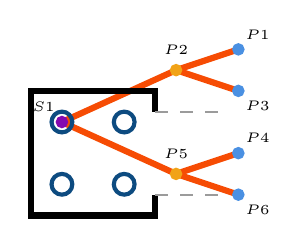
\begin{tikzpicture}[x=0.75pt,y=0.75pt,yscale=-1,xscale=1]
%uncomment if require: \path (0,182); %set diagram left start at 0, and has height of 182

%Straight Lines [id:da47465656152714486] 
\draw [color={rgb, 255:red, 246; green, 76; blue, 4 }  ,draw opacity=1 ][line width=2.25]    (315,75) -- (370,50) ;
%Shape: Square [id:dp7338884259497895] 
\draw  [line width=2.25]  (300,60) -- (360,60) -- (360,120) -- (300,120) -- cycle ;
%Straight Lines [id:da6927342142359094] 
\draw [color={rgb, 255:red, 255; green, 255; blue, 255 }  ,draw opacity=1 ][line width=3]    (360,70) -- (360,110) ;

%Straight Lines [id:da6098087629891208] 
\draw [color={rgb, 255:red, 246; green, 76; blue, 4 }  ,draw opacity=1 ][line width=2.25]    (370,50) -- (400,60) ;
%Straight Lines [id:da9586171017662504] 
\draw [color={rgb, 255:red, 246; green, 76; blue, 4 }  ,draw opacity=1 ][line width=2.25]    (400,40) -- (370,50) ;
%Straight Lines [id:da9166685119570428] 
\draw [color={rgb, 255:red, 246; green, 76; blue, 4 }  ,draw opacity=1 ][line width=2.25]    (370,100) -- (400,110) ;
%Straight Lines [id:da12081008351293132] 
\draw [color={rgb, 255:red, 246; green, 76; blue, 4 }  ,draw opacity=1 ][line width=2.25]    (315,75) -- (370,100) ;
%Straight Lines [id:da43191174777453967] 
\draw [color={rgb, 255:red, 246; green, 76; blue, 4 }  ,draw opacity=1 ][line width=2.25]    (400,90) -- (370,100) ;
%Shape: Circle [id:dp41145059566786146] 
\draw  [color={rgb, 255:red, 132; green, 9; blue, 175 }  ,draw opacity=1 ][fill={rgb, 255:red, 132; green, 9; blue, 175 }  ,fill opacity=1 ] (312.5,75) .. controls (312.5,73.62) and (313.62,72.5) .. (315,72.5) .. controls (316.38,72.5) and (317.5,73.62) .. (317.5,75) .. controls (317.5,76.38) and (316.38,77.5) .. (315,77.5) .. controls (313.62,77.5) and (312.5,76.38) .. (312.5,75) -- cycle ;
%Shape: Circle [id:dp5320458710332802] 
\draw  [color={rgb, 255:red, 13; green, 75; blue, 128 }  ,draw opacity=1 ][line width=1.5]  (310,75) .. controls (310,72.24) and (312.24,70) .. (315,70) .. controls (317.76,70) and (320,72.24) .. (320,75) .. controls (320,77.76) and (317.76,80) .. (315,80) .. controls (312.24,80) and (310,77.76) .. (310,75) -- cycle ;
%Shape: Circle [id:dp3617334287188755] 
\draw  [color={rgb, 255:red, 13; green, 75; blue, 128 }  ,draw opacity=1 ][line width=1.5]  (310,105) .. controls (310,102.24) and (312.24,100) .. (315,100) .. controls (317.76,100) and (320,102.24) .. (320,105) .. controls (320,107.76) and (317.76,110) .. (315,110) .. controls (312.24,110) and (310,107.76) .. (310,105) -- cycle ;
%Shape: Circle [id:dp07731016955749404] 
\draw  [color={rgb, 255:red, 13; green, 75; blue, 128 }  ,draw opacity=1 ][line width=1.5]  (340,105) .. controls (340,102.24) and (342.24,100) .. (345,100) .. controls (347.76,100) and (350,102.24) .. (350,105) .. controls (350,107.76) and (347.76,110) .. (345,110) .. controls (342.24,110) and (340,107.76) .. (340,105) -- cycle ;
%Shape: Circle [id:dp16339127645713447] 
\draw  [color={rgb, 255:red, 13; green, 75; blue, 128 }  ,draw opacity=1 ][line width=1.5]  (340,75) .. controls (340,72.24) and (342.24,70) .. (345,70) .. controls (347.76,70) and (350,72.24) .. (350,75) .. controls (350,77.76) and (347.76,80) .. (345,80) .. controls (342.24,80) and (340,77.76) .. (340,75) -- cycle ;
%Straight Lines [id:da6337075775283348] 
\draw [color={rgb, 255:red, 155; green, 155; blue, 155 }  ,draw opacity=1 ] [dash pattern={on 4.5pt off 4.5pt}]  (360,70) -- (390,70) ;
%Straight Lines [id:da4062260044648891] 
\draw [color={rgb, 255:red, 155; green, 155; blue, 155 }  ,draw opacity=1 ] [dash pattern={on 4.5pt off 4.5pt}]  (360,110) -- (390,110) ;
%Shape: Circle [id:dp34879830519151855] 
\draw  [color={rgb, 255:red, 74; green, 144; blue, 226 }  ,draw opacity=1 ][fill={rgb, 255:red, 74; green, 144; blue, 226 }  ,fill opacity=1 ] (397.5,110) .. controls (397.5,108.62) and (398.62,107.5) .. (400,107.5) .. controls (401.38,107.5) and (402.5,108.62) .. (402.5,110) .. controls (402.5,111.38) and (401.38,112.5) .. (400,112.5) .. controls (398.62,112.5) and (397.5,111.38) .. (397.5,110) -- cycle ;
%Shape: Circle [id:dp05200913272998542] 
\draw  [color={rgb, 255:red, 241; green, 163; blue, 23 }  ,draw opacity=1 ][fill={rgb, 255:red, 241; green, 163; blue, 23 }  ,fill opacity=1 ] (367.5,100) .. controls (367.5,98.62) and (368.62,97.5) .. (370,97.5) .. controls (371.38,97.5) and (372.5,98.62) .. (372.5,100) .. controls (372.5,101.38) and (371.38,102.5) .. (370,102.5) .. controls (368.62,102.5) and (367.5,101.38) .. (367.5,100) -- cycle ;
%Shape: Circle [id:dp43357034961897] 
\draw  [color={rgb, 255:red, 74; green, 144; blue, 226 }  ,draw opacity=1 ][fill={rgb, 255:red, 74; green, 144; blue, 226 }  ,fill opacity=1 ] (397.5,40) .. controls (397.5,38.62) and (398.62,37.5) .. (400,37.5) .. controls (401.38,37.5) and (402.5,38.62) .. (402.5,40) .. controls (402.5,41.38) and (401.38,42.5) .. (400,42.5) .. controls (398.62,42.5) and (397.5,41.38) .. (397.5,40) -- cycle ;
%Shape: Circle [id:dp7842924247669173] 
\draw  [color={rgb, 255:red, 241; green, 163; blue, 23 }  ,draw opacity=1 ][fill={rgb, 255:red, 241; green, 163; blue, 23 }  ,fill opacity=1 ] (367.5,50) .. controls (367.5,48.62) and (368.62,47.5) .. (370,47.5) .. controls (371.38,47.5) and (372.5,48.62) .. (372.5,50) .. controls (372.5,51.38) and (371.38,52.5) .. (370,52.5) .. controls (368.62,52.5) and (367.5,51.38) .. (367.5,50) -- cycle ;
%Shape: Circle [id:dp5315495156196338] 
\draw  [color={rgb, 255:red, 74; green, 144; blue, 226 }  ,draw opacity=1 ][fill={rgb, 255:red, 74; green, 144; blue, 226 }  ,fill opacity=1 ] (397.5,60) .. controls (397.5,58.62) and (398.62,57.5) .. (400,57.5) .. controls (401.38,57.5) and (402.5,58.62) .. (402.5,60) .. controls (402.5,61.38) and (401.38,62.5) .. (400,62.5) .. controls (398.62,62.5) and (397.5,61.38) .. (397.5,60) -- cycle ;
%Shape: Circle [id:dp9788740260400791] 
\draw  [color={rgb, 255:red, 74; green, 144; blue, 226 }  ,draw opacity=1 ][fill={rgb, 255:red, 74; green, 144; blue, 226 }  ,fill opacity=1 ] (397.5,90) .. controls (397.5,88.62) and (398.62,87.5) .. (400,87.5) .. controls (401.38,87.5) and (402.5,88.62) .. (402.5,90) .. controls (402.5,91.38) and (401.38,92.5) .. (400,92.5) .. controls (398.62,92.5) and (397.5,91.38) .. (397.5,90) -- cycle ;

% Text Node
\draw (313,71.6) node [anchor=south east] [inner sep=0.75pt]  [font=\tiny]  {$S1$};
% Text Node
\draw (370,44.1) node [anchor=south] [inner sep=0.75pt]  [font=\tiny]  {$P2$};
% Text Node
\draw (402,36.6) node [anchor=south west] [inner sep=0.75pt]  [font=\tiny]  {$P1$};
% Text Node
\draw (402,63.4) node [anchor=north west][inner sep=0.75pt]  [font=\tiny]  {$P3$};
% Text Node
\draw (402,86.6) node [anchor=south west] [inner sep=0.75pt]  [font=\tiny]  {$P4$};
% Text Node
\draw (370,94.1) node [anchor=south] [inner sep=0.75pt]  [font=\tiny]  {$P5$};
% Text Node
\draw (402,113.4) node [anchor=north west][inner sep=0.75pt]  [font=\tiny]  {$P6$};


\end{tikzpicture}
        \vspace{-1cm}
        \caption{Outcome state after implementing \cref{eq:tree_implementation}}
        \label{fig:final_tree_implementation}
    \end{minipage}
    \hspace{1cm}
    \begin{minipage}{0.45\textwidth}
        \centering
        

\tikzset{every picture/.style={line width=0.75pt}} %set default line width to 0.75pt        

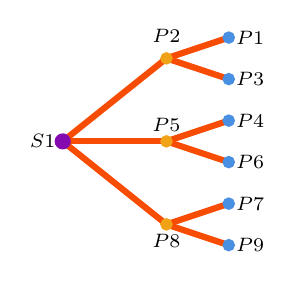
\begin{tikzpicture}[x=0.75pt,y=0.75pt,yscale=-1,xscale=1]
%uncomment if require: \path (0,182); %set diagram left start at 0, and has height of 182

%Straight Lines [id:da5808000645086375] 
\draw [color={rgb, 255:red, 246; green, 76; blue, 4 }  ,draw opacity=1 ][line width=2.25]    (360,70) -- (390,80) ;
%Straight Lines [id:da18975921226163972] 
\draw [color={rgb, 255:red, 246; green, 76; blue, 4 }  ,draw opacity=1 ][line width=2.25]    (390,60) -- (360,70) ;
%Straight Lines [id:da6595221878479601] 
\draw [color={rgb, 255:red, 246; green, 76; blue, 4 }  ,draw opacity=1 ][line width=2.25]    (360,110) -- (390,120) ;
%Straight Lines [id:da5683498370526975] 
\draw [color={rgb, 255:red, 246; green, 76; blue, 4 }  ,draw opacity=1 ][line width=2.25]    (390,100) -- (360,110) ;
%Straight Lines [id:da9165166451633462] 
\draw [color={rgb, 255:red, 246; green, 76; blue, 4 }  ,draw opacity=1 ][line width=2.25]    (360,30) -- (390,40) ;
%Straight Lines [id:da7926013585642647] 
\draw [color={rgb, 255:red, 246; green, 76; blue, 4 }  ,draw opacity=1 ][line width=2.25]    (390,20) -- (360,30) ;
%Straight Lines [id:da7417109803866969] 
\draw [color={rgb, 255:red, 246; green, 76; blue, 4 }  ,draw opacity=1 ][line width=2.25]    (310,70) -- (360,30) ;
%Straight Lines [id:da32862812153335397] 
\draw [color={rgb, 255:red, 246; green, 76; blue, 4 }  ,draw opacity=1 ][line width=2.25]    (310,70) -- (360,70) ;
%Straight Lines [id:da9935618987409959] 
\draw [color={rgb, 255:red, 246; green, 76; blue, 4 }  ,draw opacity=1 ][line width=2.25]    (310,70) -- (360,110) ;
%Shape: Circle [id:dp31789546772639043] 
\draw  [color={rgb, 255:red, 132; green, 9; blue, 175 }  ,draw opacity=1 ][fill={rgb, 255:red, 132; green, 9; blue, 175 }  ,fill opacity=1 ] (306.63,70) .. controls (306.63,68.14) and (308.14,66.63) .. (310,66.63) .. controls (311.86,66.63) and (313.38,68.14) .. (313.38,70) .. controls (313.38,71.86) and (311.86,73.38) .. (310,73.38) .. controls (308.14,73.38) and (306.63,71.86) .. (306.63,70) -- cycle ;
%Shape: Circle [id:dp6750291852439366] 
\draw  [color={rgb, 255:red, 74; green, 144; blue, 226 }  ,draw opacity=1 ][fill={rgb, 255:red, 74; green, 144; blue, 226 }  ,fill opacity=1 ] (387.5,120) .. controls (387.5,118.62) and (388.62,117.5) .. (390,117.5) .. controls (391.38,117.5) and (392.5,118.62) .. (392.5,120) .. controls (392.5,121.38) and (391.38,122.5) .. (390,122.5) .. controls (388.62,122.5) and (387.5,121.38) .. (387.5,120) -- cycle ;
%Shape: Circle [id:dp5494552717190384] 
\draw  [color={rgb, 255:red, 241; green, 163; blue, 23 }  ,draw opacity=1 ][fill={rgb, 255:red, 241; green, 163; blue, 23 }  ,fill opacity=1 ] (357.5,110) .. controls (357.5,108.62) and (358.62,107.5) .. (360,107.5) .. controls (361.38,107.5) and (362.5,108.62) .. (362.5,110) .. controls (362.5,111.38) and (361.38,112.5) .. (360,112.5) .. controls (358.62,112.5) and (357.5,111.38) .. (357.5,110) -- cycle ;
%Shape: Circle [id:dp8629159729730512] 
\draw  [color={rgb, 255:red, 74; green, 144; blue, 226 }  ,draw opacity=1 ][fill={rgb, 255:red, 74; green, 144; blue, 226 }  ,fill opacity=1 ] (387.5,80) .. controls (387.5,78.62) and (388.62,77.5) .. (390,77.5) .. controls (391.38,77.5) and (392.5,78.62) .. (392.5,80) .. controls (392.5,81.38) and (391.38,82.5) .. (390,82.5) .. controls (388.62,82.5) and (387.5,81.38) .. (387.5,80) -- cycle ;
%Shape: Circle [id:dp6642418585732942] 
\draw  [color={rgb, 255:red, 241; green, 163; blue, 23 }  ,draw opacity=1 ][fill={rgb, 255:red, 241; green, 163; blue, 23 }  ,fill opacity=1 ] (357.5,70) .. controls (357.5,68.62) and (358.62,67.5) .. (360,67.5) .. controls (361.38,67.5) and (362.5,68.62) .. (362.5,70) .. controls (362.5,71.38) and (361.38,72.5) .. (360,72.5) .. controls (358.62,72.5) and (357.5,71.38) .. (357.5,70) -- cycle ;
%Shape: Circle [id:dp6409499135433837] 
\draw  [color={rgb, 255:red, 74; green, 144; blue, 226 }  ,draw opacity=1 ][fill={rgb, 255:red, 74; green, 144; blue, 226 }  ,fill opacity=1 ] (387.5,60) .. controls (387.5,58.62) and (388.62,57.5) .. (390,57.5) .. controls (391.38,57.5) and (392.5,58.62) .. (392.5,60) .. controls (392.5,61.38) and (391.38,62.5) .. (390,62.5) .. controls (388.62,62.5) and (387.5,61.38) .. (387.5,60) -- cycle ;
%Shape: Circle [id:dp6267335925860115] 
\draw  [color={rgb, 255:red, 74; green, 144; blue, 226 }  ,draw opacity=1 ][fill={rgb, 255:red, 74; green, 144; blue, 226 }  ,fill opacity=1 ] (387.5,100) .. controls (387.5,98.62) and (388.62,97.5) .. (390,97.5) .. controls (391.38,97.5) and (392.5,98.62) .. (392.5,100) .. controls (392.5,101.38) and (391.38,102.5) .. (390,102.5) .. controls (388.62,102.5) and (387.5,101.38) .. (387.5,100) -- cycle ;
%Shape: Circle [id:dp35239961388070173] 
\draw  [color={rgb, 255:red, 74; green, 144; blue, 226 }  ,draw opacity=1 ][fill={rgb, 255:red, 74; green, 144; blue, 226 }  ,fill opacity=1 ] (387.5,40) .. controls (387.5,38.62) and (388.62,37.5) .. (390,37.5) .. controls (391.38,37.5) and (392.5,38.62) .. (392.5,40) .. controls (392.5,41.38) and (391.38,42.5) .. (390,42.5) .. controls (388.62,42.5) and (387.5,41.38) .. (387.5,40) -- cycle ;
%Shape: Circle [id:dp6520996479300846] 
\draw  [color={rgb, 255:red, 241; green, 163; blue, 23 }  ,draw opacity=1 ][fill={rgb, 255:red, 241; green, 163; blue, 23 }  ,fill opacity=1 ] (357.5,30) .. controls (357.5,28.62) and (358.62,27.5) .. (360,27.5) .. controls (361.38,27.5) and (362.5,28.62) .. (362.5,30) .. controls (362.5,31.38) and (361.38,32.5) .. (360,32.5) .. controls (358.62,32.5) and (357.5,31.38) .. (357.5,30) -- cycle ;
%Shape: Circle [id:dp39086329664120045] 
\draw  [color={rgb, 255:red, 74; green, 144; blue, 226 }  ,draw opacity=1 ][fill={rgb, 255:red, 74; green, 144; blue, 226 }  ,fill opacity=1 ] (387.5,20) .. controls (387.5,18.62) and (388.62,17.5) .. (390,17.5) .. controls (391.38,17.5) and (392.5,18.62) .. (392.5,20) .. controls (392.5,21.38) and (391.38,22.5) .. (390,22.5) .. controls (388.62,22.5) and (387.5,21.38) .. (387.5,20) -- cycle ;

% Text Node
\draw (308,70) node [anchor=east] [inner sep=0.75pt]  [font=\scriptsize]  {$S1$};
% Text Node
\draw (392,20) node [anchor=west] [inner sep=0.75pt]  [font=\scriptsize]  {$P1$};
% Text Node
\draw (392,40) node [anchor=west] [inner sep=0.75pt]  [font=\scriptsize]  {$P3$};
% Text Node
\draw (360,24.1) node [anchor=south] [inner sep=0.75pt]  [font=\scriptsize]  {$P2$};
% Text Node
\draw (392,60) node [anchor=west] [inner sep=0.75pt]  [font=\scriptsize]  {$P4$};
% Text Node
\draw (392,80) node [anchor=west] [inner sep=0.75pt]  [font=\scriptsize]  {$P6$};
% Text Node
\draw (392,100) node [anchor=west] [inner sep=0.75pt]  [font=\scriptsize]  {$P7$};
% Text Node
\draw (392,120) node [anchor=west] [inner sep=0.75pt]  [font=\scriptsize]  {$P9$};
% Text Node
\draw (360,66.6) node [anchor=south] [inner sep=0.75pt]  [font=\scriptsize]  {$P5$};
% Text Node
\draw (360,113.4) node [anchor=north] [inner sep=0.75pt]  [font=\scriptsize]  {$P8$};


\end{tikzpicture}
        \vspace{-1cm}
        \caption{$(3, 2)$ tree graph state}
        \label{fig:3_3_tree}
    \end{minipage}
\end{figure}
\section{(n, 2) Tree Graph State}
\label{sec:n_2_tree}

Beginning from the final state derived from \cref{eq:tree_implementation}, by replicating the process outlined in \cref{eq:1_branch_implementation} to generate another branch, we could extend the implementation to create a generalized $(2, 2)$ tree graph state, thereby enabling the implementation of a $(n, 2)$ tree state.

As an example let us consider a $(3, 2)$ tree state (figure 1).
It can be implemented using the following sequence of gates.
\begin{equation}
    \begin{quantikz}[column sep=0.2cm]
      & \gate{Y_+} & \qw & \qw & \ctrl{1} & \qw & \qw & \qw & \qw & \qw & \qw & \ctrl{1} & \qw & \qw & \qw & \qw & \qw & \qw & \ctrl{1} & \qw & \qw & \qw  \\
      & \gate{Y_+} & \ctrl{3} & \gate{Y_-} & \control{} & \ctrl{2} & \gate{Y_+} & \swap{1} & \gate{Y_+} & \ctrl{6} & \gate{Y_-} & \control{} & \ctrl{5} & \gate{Y_+} & \swap{4} & \gate{Y_+} & \ctrl{8} & \gate{Y_-} & \control{} & \ctrl{7} & \gate{Y_+} & \qw  \\
      & \qw & \qw & \qw & \qw & \qw & \qw & \targX{} & \qw & \qw & \qw & \qw & \qw & \qw & \qw & \qw & \qw & \qw & \qw & \qw & \qw & \qw  \\
      & \qw & \qw & \qw & \qw & \targ{} & \qw & \qw & \qw & \qw & \qw & \qw & \qw & \qw & \qw & \qw & \qw & \qw & \qw & \qw & \qw & \qw  \\
      & \qw & \targ{} & \qw & \qw & \qw & \qw & \qw & \qw & \qw & \qw & \qw & \qw & \qw & \qw & \qw & \qw & \qw & \qw & \qw & \qw & \qw  \\
      & \qw & \qw & \qw & \qw & \qw & \qw & \qw & \qw & \qw & \qw & \qw & \qw & \qw & \targX{} & \qw & \qw & \qw & \qw & \qw & \qw & \qw  \\
      & \qw & \qw & \qw & \qw & \qw & \qw & \qw & \qw & \qw & \qw & \qw & \targ{} & \qw & \qw & \qw & \qw & \qw & \qw & \qw & \qw & \qw \\
      & \qw & \qw & \qw & \qw & \qw & \qw & \qw & \qw & \targ{} & \qw & \qw & \qw & \qw & \qw & \qw & \qw & \qw & \qw & \qw & \qw & \qw  \\
      & \qw & \qw & \qw & \qw & \qw & \qw & \qw & \qw & \qw & \qw & \qw & \qw & \qw & \qw & \qw & \qw & \qw & \qw & \targ{} & \qw & \qw  \\
      & \qw & \qw & \qw & \qw & \qw & \qw & \qw & \qw & \qw & \qw & \qw & \qw & \qw & \qw & \qw & \targ{} & \qw & \qw & \qw & \qw & \qw 
    \end{quantikz}
    \notag
\end{equation}

Although the initial state of all qubits in the protocol remains $\ket{0}$, for the sake of fitting the circuit within the page, we imply their initialization.

%\begin{figure}
%    \centering
%    

\tikzset{every picture/.style={line width=0.75pt}} %set default line width to 0.75pt        

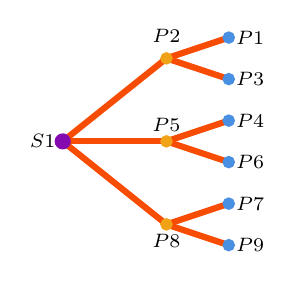
\begin{tikzpicture}[x=0.75pt,y=0.75pt,yscale=-1,xscale=1]
%uncomment if require: \path (0,182); %set diagram left start at 0, and has height of 182

%Straight Lines [id:da5808000645086375] 
\draw [color={rgb, 255:red, 246; green, 76; blue, 4 }  ,draw opacity=1 ][line width=2.25]    (360,70) -- (390,80) ;
%Straight Lines [id:da18975921226163972] 
\draw [color={rgb, 255:red, 246; green, 76; blue, 4 }  ,draw opacity=1 ][line width=2.25]    (390,60) -- (360,70) ;
%Straight Lines [id:da6595221878479601] 
\draw [color={rgb, 255:red, 246; green, 76; blue, 4 }  ,draw opacity=1 ][line width=2.25]    (360,110) -- (390,120) ;
%Straight Lines [id:da5683498370526975] 
\draw [color={rgb, 255:red, 246; green, 76; blue, 4 }  ,draw opacity=1 ][line width=2.25]    (390,100) -- (360,110) ;
%Straight Lines [id:da9165166451633462] 
\draw [color={rgb, 255:red, 246; green, 76; blue, 4 }  ,draw opacity=1 ][line width=2.25]    (360,30) -- (390,40) ;
%Straight Lines [id:da7926013585642647] 
\draw [color={rgb, 255:red, 246; green, 76; blue, 4 }  ,draw opacity=1 ][line width=2.25]    (390,20) -- (360,30) ;
%Straight Lines [id:da7417109803866969] 
\draw [color={rgb, 255:red, 246; green, 76; blue, 4 }  ,draw opacity=1 ][line width=2.25]    (310,70) -- (360,30) ;
%Straight Lines [id:da32862812153335397] 
\draw [color={rgb, 255:red, 246; green, 76; blue, 4 }  ,draw opacity=1 ][line width=2.25]    (310,70) -- (360,70) ;
%Straight Lines [id:da9935618987409959] 
\draw [color={rgb, 255:red, 246; green, 76; blue, 4 }  ,draw opacity=1 ][line width=2.25]    (310,70) -- (360,110) ;
%Shape: Circle [id:dp31789546772639043] 
\draw  [color={rgb, 255:red, 132; green, 9; blue, 175 }  ,draw opacity=1 ][fill={rgb, 255:red, 132; green, 9; blue, 175 }  ,fill opacity=1 ] (306.63,70) .. controls (306.63,68.14) and (308.14,66.63) .. (310,66.63) .. controls (311.86,66.63) and (313.38,68.14) .. (313.38,70) .. controls (313.38,71.86) and (311.86,73.38) .. (310,73.38) .. controls (308.14,73.38) and (306.63,71.86) .. (306.63,70) -- cycle ;
%Shape: Circle [id:dp6750291852439366] 
\draw  [color={rgb, 255:red, 74; green, 144; blue, 226 }  ,draw opacity=1 ][fill={rgb, 255:red, 74; green, 144; blue, 226 }  ,fill opacity=1 ] (387.5,120) .. controls (387.5,118.62) and (388.62,117.5) .. (390,117.5) .. controls (391.38,117.5) and (392.5,118.62) .. (392.5,120) .. controls (392.5,121.38) and (391.38,122.5) .. (390,122.5) .. controls (388.62,122.5) and (387.5,121.38) .. (387.5,120) -- cycle ;
%Shape: Circle [id:dp5494552717190384] 
\draw  [color={rgb, 255:red, 241; green, 163; blue, 23 }  ,draw opacity=1 ][fill={rgb, 255:red, 241; green, 163; blue, 23 }  ,fill opacity=1 ] (357.5,110) .. controls (357.5,108.62) and (358.62,107.5) .. (360,107.5) .. controls (361.38,107.5) and (362.5,108.62) .. (362.5,110) .. controls (362.5,111.38) and (361.38,112.5) .. (360,112.5) .. controls (358.62,112.5) and (357.5,111.38) .. (357.5,110) -- cycle ;
%Shape: Circle [id:dp8629159729730512] 
\draw  [color={rgb, 255:red, 74; green, 144; blue, 226 }  ,draw opacity=1 ][fill={rgb, 255:red, 74; green, 144; blue, 226 }  ,fill opacity=1 ] (387.5,80) .. controls (387.5,78.62) and (388.62,77.5) .. (390,77.5) .. controls (391.38,77.5) and (392.5,78.62) .. (392.5,80) .. controls (392.5,81.38) and (391.38,82.5) .. (390,82.5) .. controls (388.62,82.5) and (387.5,81.38) .. (387.5,80) -- cycle ;
%Shape: Circle [id:dp6642418585732942] 
\draw  [color={rgb, 255:red, 241; green, 163; blue, 23 }  ,draw opacity=1 ][fill={rgb, 255:red, 241; green, 163; blue, 23 }  ,fill opacity=1 ] (357.5,70) .. controls (357.5,68.62) and (358.62,67.5) .. (360,67.5) .. controls (361.38,67.5) and (362.5,68.62) .. (362.5,70) .. controls (362.5,71.38) and (361.38,72.5) .. (360,72.5) .. controls (358.62,72.5) and (357.5,71.38) .. (357.5,70) -- cycle ;
%Shape: Circle [id:dp6409499135433837] 
\draw  [color={rgb, 255:red, 74; green, 144; blue, 226 }  ,draw opacity=1 ][fill={rgb, 255:red, 74; green, 144; blue, 226 }  ,fill opacity=1 ] (387.5,60) .. controls (387.5,58.62) and (388.62,57.5) .. (390,57.5) .. controls (391.38,57.5) and (392.5,58.62) .. (392.5,60) .. controls (392.5,61.38) and (391.38,62.5) .. (390,62.5) .. controls (388.62,62.5) and (387.5,61.38) .. (387.5,60) -- cycle ;
%Shape: Circle [id:dp6267335925860115] 
\draw  [color={rgb, 255:red, 74; green, 144; blue, 226 }  ,draw opacity=1 ][fill={rgb, 255:red, 74; green, 144; blue, 226 }  ,fill opacity=1 ] (387.5,100) .. controls (387.5,98.62) and (388.62,97.5) .. (390,97.5) .. controls (391.38,97.5) and (392.5,98.62) .. (392.5,100) .. controls (392.5,101.38) and (391.38,102.5) .. (390,102.5) .. controls (388.62,102.5) and (387.5,101.38) .. (387.5,100) -- cycle ;
%Shape: Circle [id:dp35239961388070173] 
\draw  [color={rgb, 255:red, 74; green, 144; blue, 226 }  ,draw opacity=1 ][fill={rgb, 255:red, 74; green, 144; blue, 226 }  ,fill opacity=1 ] (387.5,40) .. controls (387.5,38.62) and (388.62,37.5) .. (390,37.5) .. controls (391.38,37.5) and (392.5,38.62) .. (392.5,40) .. controls (392.5,41.38) and (391.38,42.5) .. (390,42.5) .. controls (388.62,42.5) and (387.5,41.38) .. (387.5,40) -- cycle ;
%Shape: Circle [id:dp6520996479300846] 
\draw  [color={rgb, 255:red, 241; green, 163; blue, 23 }  ,draw opacity=1 ][fill={rgb, 255:red, 241; green, 163; blue, 23 }  ,fill opacity=1 ] (357.5,30) .. controls (357.5,28.62) and (358.62,27.5) .. (360,27.5) .. controls (361.38,27.5) and (362.5,28.62) .. (362.5,30) .. controls (362.5,31.38) and (361.38,32.5) .. (360,32.5) .. controls (358.62,32.5) and (357.5,31.38) .. (357.5,30) -- cycle ;
%Shape: Circle [id:dp39086329664120045] 
\draw  [color={rgb, 255:red, 74; green, 144; blue, 226 }  ,draw opacity=1 ][fill={rgb, 255:red, 74; green, 144; blue, 226 }  ,fill opacity=1 ] (387.5,20) .. controls (387.5,18.62) and (388.62,17.5) .. (390,17.5) .. controls (391.38,17.5) and (392.5,18.62) .. (392.5,20) .. controls (392.5,21.38) and (391.38,22.5) .. (390,22.5) .. controls (388.62,22.5) and (387.5,21.38) .. (387.5,20) -- cycle ;

% Text Node
\draw (308,70) node [anchor=east] [inner sep=0.75pt]  [font=\scriptsize]  {$S1$};
% Text Node
\draw (392,20) node [anchor=west] [inner sep=0.75pt]  [font=\scriptsize]  {$P1$};
% Text Node
\draw (392,40) node [anchor=west] [inner sep=0.75pt]  [font=\scriptsize]  {$P3$};
% Text Node
\draw (360,24.1) node [anchor=south] [inner sep=0.75pt]  [font=\scriptsize]  {$P2$};
% Text Node
\draw (392,60) node [anchor=west] [inner sep=0.75pt]  [font=\scriptsize]  {$P4$};
% Text Node
\draw (392,80) node [anchor=west] [inner sep=0.75pt]  [font=\scriptsize]  {$P6$};
% Text Node
\draw (392,100) node [anchor=west] [inner sep=0.75pt]  [font=\scriptsize]  {$P7$};
% Text Node
\draw (392,120) node [anchor=west] [inner sep=0.75pt]  [font=\scriptsize]  {$P9$};
% Text Node
\draw (360,66.6) node [anchor=south] [inner sep=0.75pt]  [font=\scriptsize]  {$P5$};
% Text Node
\draw (360,113.4) node [anchor=north] [inner sep=0.75pt]  [font=\scriptsize]  {$P8$};


\end{tikzpicture}
%    \vspace{-1cm}
%    \caption{$(3, 2)$ tree graph state}
%    \label{fig:3_3_tree}
%\end{figure}
%
%\section{(n, 3) Tree Graph State}